% =============================================================================
%  Paper A — Supplementary Information
%
%  Results moved out of the main text for length. Every number is MEASURED and
%  cites an on-disk artifact, exactly as in the main text (AGENTS.md §5.2).
% =============================================================================

\documentclass[11pt]{article}

\usepackage[T1]{fontenc}
\usepackage{amsmath,amssymb}
\usepackage{graphicx}
\graphicspath{{figures/}{./}}
\usepackage{booktabs}
\usepackage[margin=1in]{geometry}
\usepackage[round,numbers]{natbib}
\bibliographystyle{unsrtnat}
\usepackage{hyperref}
\usepackage{xcolor}

\newcommand{\MEASURED}{\textbf{MEASURED}}

\title{Supplementary Information:\\
Few-shot metal adaptation recovers cross-metal collapse}
\author{Hugo Lee \and Mol-Metal contributors}
\date{\today}

\begin{document}
\maketitle

\section{Probe-cohort collapse decomposition}
\label{sec:si:decomp}

The main text reports the collapse on the paper-funnel cohort. On an earlier,
smaller probe cohort (rows filtered to $\leq24$\,h exposure) the collapse is
larger and we additionally measured a same-metal Bemis--Murcko scaffold-split
control, which separates the metal axis from the ordinary novel-scaffold
penalty.

\begin{table}[h]
\centering
\caption{Probe-cohort transfer decomposition: within-metal 5-fold, same-metal
scaffold split, and cross-metal LOMO, same scorer. Net metal $=$ scaffold
$-$ cross. \MEASURED:
\texttt{metrics/by\_metric/metal\_activity\_transfer\_seed\_stability.json},
\texttt{metal\_activity\_transfer\_scaffold.json}.}
\begin{tabular}{lcccc}
\toprule
Metal & Within (5-fold) & Scaffold & Cross (LOMO) & Net metal \\
\midrule
Ru & $0.8271$ $[0.8128, 0.8363]$ & $0.7338$ & $0.6179$ & $+0.116$ \\
Ir & $0.8430$ $[0.8295, 0.8597]$ & $0.7087$ & $0.5276$ & $+0.181$ \\
Rh & $0.6974$ $[0.6429, 0.7381]$ & $0.4690$ & $0.5190$ & $-0.050$ \\
Os & $0.4960$ $[0.3133, 0.5867]$ & $0.4900$ & $0.4950$ & $-0.005$ \\
Re & $0.9480$ $[0.9083, 0.9819]$ & $0.8465$ & $0.4429$ & $+0.404$ \\
\bottomrule
\end{tabular}
\end{table}

A same-metal scaffold split costs $0.10$--$0.12$ on the two metals where the
penalty resolves, so roughly half of the raw within-to-cross drop is ordinary
novel-scaffold generalisation and the metal axis is the largest single remaining
shift. On this smaller cohort Rh ($n=51$), Os ($n=36$) and Re ($n=74$) are too
small to gate: a label-permutation null on the fixed cross-metal ranking places
all three inside the null (null SD $\pm0.09$--$0.10$), and only Ru is
significantly above chance after Holm correction. This is the reason the main
text adopts the paper-funnel cohort, where every metal is resolvable.
\MEASURED: \texttt{metrics/by\_metric/metal\_activity\_transfer\_permutation\_null.json},
\texttt{metal\_activity\_transfer\_significance.json}.

\paragraph{Representation-dependence.} Replacing the fingerprint scorer with the
chemprop~v2 backbone on the probe cohort reproduces the collapse for Ru, Ir and
Rh and recovers Re ($0.7368$, Holm $p=0.010$), where the fingerprint scores
$0.4429$. Whether Re transfers is therefore a property of the representation,
not of the metal axis. \MEASURED:
\texttt{metrics/by\_metric/pa3\_chemprop\_lomo\_probe\_cohort.json}.

\section{Static metal conditioning does not repair the collapse}
\label{sec:si:metalcond}

The main text's repair is adaptation. The obvious alternative --- feeding metal
identity into a zero-shot model --- does not work, and this is the control that
motivates the adaptation framing.

\begin{table}[h]
\centering
\caption{Static metal conditioning, cross-metal LOMO mean over five metals,
paired against the unconditioned baseline. \MEASURED:
\texttt{metrics/by\_metric/pa15\_metalcond\_lomo.json},
\texttt{l3\_metalcond\_lomo.json}.}
\begin{tabular}{lccc}
\toprule
Arm & Cross-metal mean & Paired $\Delta$ & Holm $p$ \\
\midrule
Unconditioned (baseline) & $0.5693$ & --- & --- \\
Metal token              & $0.5205$ & $-0.0488$ & $1.000$ \\
Metal descriptor         & $0.5480$ & $-0.0215$ & $1.000$ \\
FiLM                     & $0.5275$ & $-0.0418$ & $0.984$ \\
\bottomrule
\end{tabular}
\end{table}

All three leave the cross-metal mean at or below the unconditioned baseline:
the collapse is not a missing-input problem.

\section{tmQM pretraining A/B}
\label{sec:si:pretrain}

\begin{table}[h]
\centering
\caption{tmQM pretraining A/B on the Ru and Ir activity heads, fixed
Bemis--Murcko scaffold split, paired over five seeds; \texttt{init} is the only
variable. \MEASURED: \texttt{metrics/by\_metric/tmqm\_pretrain\_init\_ab\_ru.json},
\texttt{tmqm\_pretrain\_init\_ab\_multimetal.json}.}
\begin{tabular}{llcc}
\toprule
Metal & Arm & Mean ROC-AUC & Sample std over seeds \\
\midrule
Ru ($n_{\text{test}}=215$) & tmQM init   & $0.7778$ & $0.0194$ \\
Ru                         & random init & $0.7872$ & $0.0201$ \\
Ir ($n_{\text{test}}=56$)  & tmQM init   & $0.7205$ & $0.0399$ \\
Ir                         & random init & $0.6719$ & $0.0258$ \\
\bottomrule
\end{tabular}
\end{table}

On Ru the paired delta is $-0.0094$ (t-based 95\% CI $[-0.0406,+0.0218]$,
$t(4)=-0.84$, $2/5$ seeds positive). On Ir the point estimate is $+0.0486$ but
it does not clear the paired $t$-test ($3/5$ seeds positive, CI
$[-0.0238,+0.1210]$ includes zero, one-sided $p=0.068$; a 5-seed percentile
bootstrap returns $p=0.012$ but is anti-conservative at that sample size).
Across the two metals no Holm-corrected effect is significant, so we make no
pretraining claim. The measurement is sound --- the paired design cancels seed
variance and both arms log the tmQM tensor-load count --- the effect is null.
An earlier $+0.0181$ came from a degenerate, molecule-level splitter and does
not survive the fix.

\begin{figure}[h]
\centering
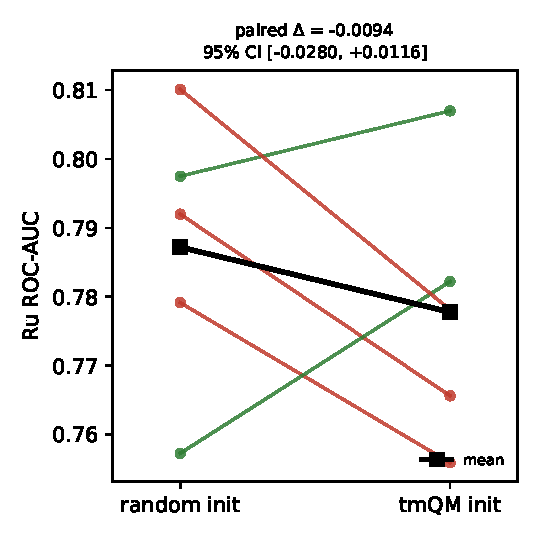
\includegraphics[width=0.55\linewidth]{si_pretrain.pdf}
\caption{Paired per-seed deltas for the tmQM pretraining A/B on the Ru arm
(fixed Bemis--Murcko scaffold split). Two of five seeds move toward tmQM
(green), three away (red); the black line is the mean. The interval crosses
zero. \MEASURED: \texttt{metrics/by\_metric/tmqm\_pretrain\_init\_ab\_ru.json}.}
\label{fig:si:pretrain}
\end{figure}

\section{MoleculeNet backbone control}
\label{sec:si:moleculenet}

The control's only job is to show the encoder is a competent organic-property
predictor, so that the cross-metal collapse is a property of the axis and not of
a backbone that cannot fit.

\begin{table}[h]
\centering
\caption{D-MPNN and chemprop~v2 on MoleculeNet tasks, identical scaffold split,
five seeds. ``Literature'' is the commonly quoted best-of-search constant.
\MEASURED: \texttt{metrics/by\_metric/moleculenet\_auc\_dmpnn\_5seed\_cap512\_d4.json},
\texttt{moleculenet\_auc\_chemprop\_v2\_same\_protocol.json}.}
\begin{tabular}{lcccc}
\toprule
Task & This work (D-MPNN $512/4$) & chemprop v2 (same protocol) & $\Delta$ & Literature \\
\midrule
bbbp    & $0.8994 \pm 0.0218$ & $0.8861 \pm 0.0135$ & $+0.0133$ & $0.940$ \\
hiv     & $0.7889 \pm 0.0189$ & $0.7807 \pm 0.0222$ & $+0.0082$ & $0.823$ \\
bace    & $0.7933 \pm 0.0250$ & $0.8458 \pm 0.0113$ & $-0.0525$ & $0.876$ \\
clintox & $0.8303 \pm 0.0133$ & $0.8847 \pm 0.0193$ & $-0.0544$ & $0.894$ \\
\midrule
mean    & $0.8280$ & $0.8493$ & $-0.0214$ & $0.8832$ \\
\bottomrule
\end{tabular}
\end{table}

The D-MPNN wins bbbp and hiv and loses bace and clintox. The two losses exceed
seed noise and are carried here rather than in the main text; they are generic
ADMET endpoints outside this paper's target chemistry and do not bear on the
metal-axis claims.

\section{Tie-rule sensitivity}
\label{sec:si:tie}

When duplicate measurements of a ligand disagree, the collapse rule resolves an
exact tie toward \emph{active}. This is the anti-conservative direction, so we
report the within-metal column under both rules.

\begin{table}[h]
\centering
\caption{Within-metal AUC under the two tie rules (probe cohort).
\MEASURED: \texttt{metrics/by\_metric/metal\_activity\_transfer\_tie\_sensitivity.json}.}
\begin{tabular}{lcc}
\toprule
 & Ties $\to$ active (current) & Ties $\to$ inactive (conservative) \\
\midrule
Ru & $0.8128$--$0.8363$ & $0.7880$--$0.8082$ \\
Ir & $0.8295$--$0.8597$ & $0.8237$--$0.8374$ \\
\midrule
\multicolumn{3}{l}{Krasnov published: Ru $0.81$, Ir $0.73$} \\
\bottomrule
\end{tabular}
\end{table}

The Ir result is robust to the rule; the Ru result is decided by it. The
collapse itself is unaffected, being a difference of two columns computed under
the same rule.

\begin{figure}[h]
\centering
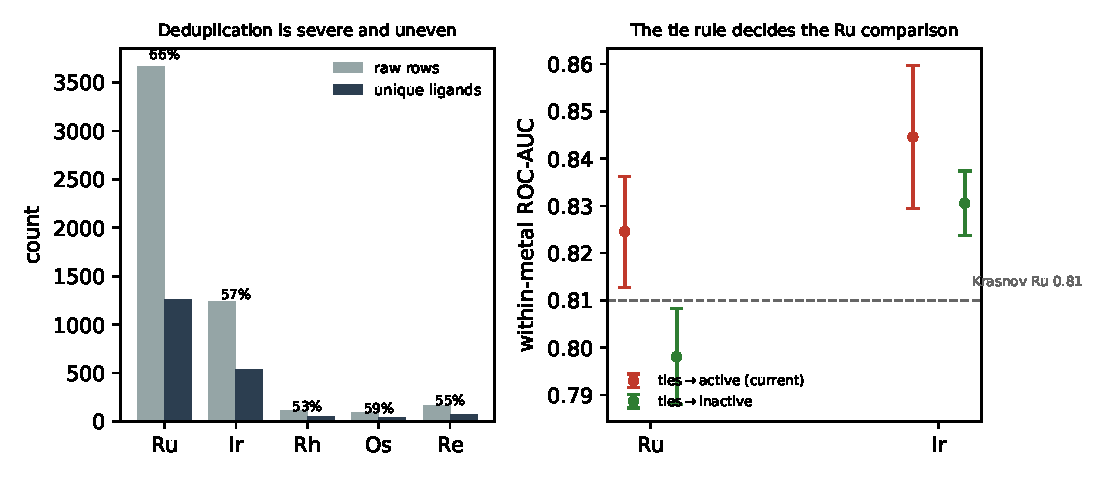
\includegraphics[width=0.95\linewidth]{si_dedup_tie.pdf}
\caption{Left: raw rows versus unique ligands per metal (percentage is the
duplication rate). Right: within-metal AUC interval across seeds under the two
tie rules; the Ru interval crosses the published $0.81$ line, the Ir interval
does not. \MEASURED:
\texttt{metrics/by\_metric/metal\_activity\_transfer\_seed\_stability.json},
\texttt{metal\_activity\_transfer\_tie\_sensitivity.json}.}
\label{fig:si:dedup}
\end{figure}

\section{Cohort-construction trap}
\label{sec:lim:cohort}

A preprocessing filter applied to an already-filtered artifact can manufacture a
below-chance result. The default probe-cohort snapshot is filtered to short
exposure times ($\leq24$\,h); raising the threshold at training time cannot
recover dropped rows, and the loaded cohort stayed byte-identical --- the filter
silently did nothing. The consequence was a below-chance fold (Rh collapsed to
$108$ test ligands, AUC $0.3812$) with no change to the model. Readers building
on MetalCytoToxDB can hit the same trap; the main text's cohort avoids it by
constructing from the raw database under the published rule.
\MEASURED: \texttt{metrics/by\_metric/metal\_lomo\_auc\_wasserstein.json}.

\section{tmQM bond-perception reference}
\label{sec:si:bond}

\begin{table}[h]
\centering
\caption{Bond perception on 900 held-out tmQM complexes, identical cohort and
per-complex aggregation for every column. \MEASURED:
\texttt{metrics/by\_metric/tmqm\_bond\_perception\_3seed.json}.}
\begin{tabular}{lccc}
\toprule
 & Learned head & OpenBabel \citep{openbabel} & RDKit (stripped) \citep{rdkit} \\
\midrule
bond EXISTENCE F1   & $\mathbf{0.9962 \pm 0.0008}$ & $0.9771$ & $0.9998$ \\
exact-type rate     & $\mathbf{0.0956 \pm 0.0113}$ & $0.0300$ & $0.0220$ \\
macro-F1(type)      & $0.4784 \pm 0.0055$ & $\mathbf{0.5051}$ & $0.2809$ \\
success rate        & $1.000$ & $1.000$ & $0.303$ \\
\bottomrule
\end{tabular}
\end{table}

The learned head wins two of three axes but loses macro-F1(type) to OpenBabel by
$0.0267$, consistent across all three seeds.

\bibliography{refs}

\end{document}
